\documentclass[10pt, conference]{IEEEtran}
\hyphenation{op-tical net-works semi-conduc-tor}
\usepackage{graphicx}
\usepackage{fancyhdr}
\usepackage{url}
\usepackage{amsmath}
\usepackage{lipsum}
\usepackage{bookmark}
\usepackage[normalem]{ulem}
\useunder{\uline}{\ul}{}
\def\code#1{\texttt{#1}}

\pagestyle{fancy}
\fancyhf{}
\lhead{\textsc{ELEN4020}}
\rhead{\textsc{Laboratory Exercise No 2}}
\rfoot{Page \thepage\ }


\begin{document}
\begin{titlepage}
\newcommand{\HRule}{\rule{\linewidth}{0.5mm}} % Defines a new command for the horizontal lines, change thickness here

\center % Center everything on the page
 
%----------------------------------------------------------------------------------------
%	HEADING SECTIONS
%----------------------------------------------------------------------------------------

\textsc{\LARGE University of Witwatersrand}\\[1.5cm] % Name of your university/college
%----------------------------------------------------------------------------------------
%	LOGO SECTION
%----------------------------------------------------------------------------------------


\includegraphics[scale=0.25]{Wits.png}% Include a department/university logo - this will require the graphicx package
 
 
%----------------------------------------------------------------------------------------
\textsc{\Large ELEN4020}\\[0.5cm] % Major heading such as course name
\textsc{\large Data Intensive Computing In Data Science}\\[0.5cm] % Minor heading such as course title



%----------------------------------------------------------------------------------------
%	TITLE SECTION
%----------------------------------------------------------------------------------------

\HRule \\[0.4cm]
{ \huge \bfseries Laboratory Exercise 2}\\[0.4cm] % Title of your document
\HRule \\[1.5cm]
 
%----------------------------------------------------------------------------------------
%	AUTHOR SECTION
%----------------------------------------------------------------------------------------

\begin{minipage}{0.4\textwidth}
\begin{flushleft} \large
	\emph{Authors:}\\
	\textsc{Kishan Narotam - 717 931\\Jesal Chana - 603 177} 
\end{flushleft}
\end{minipage}
~
\begin{minipage}{0.4\textwidth}
\begin{flushright} \large
	\emph{Authors:} \\
	\textsc{Syed Hussain - 600 524\\Yusuf Ally - 604 973} 
\end{flushright}
\end{minipage}\\[2cm]

%----------------------------------------------------------------------------------------
%	DATE SECTION
%----------------------------------------------------------------------------------------

{\large 9\textsuperscript{th} March 2018}\\[2cm] % Date, change the \today to a set date if you want to be precise

%-------------------------------------------------------------------------------------

\vfill % Fill the rest of the page with whitespace

\end{titlepage}
%----------------------------------------------------------------------------------------


%----------------------------------------------------------------------------------------
%	MAIN BODY OF REPORT
%----------------------------------------------------------------------------------------

\section{Problem Description}
\label{Problem Description}
A square matrix, defined as $A[N_0][N_1]$, must be created with various dimensions, where $N_0 = N_1 = 128, 1024,8192$. The matrix could be an integer which is 4 bytes or a short floating point which too is 4 bytes. The elements of the matrix must be generated using the formula presented in equation~\ref{eqn1}:
\begin{equation}
\label{eqn1}
\begin{split}
A\langle i, j\rangle & = i *N_j + j
\end{split}
\end{equation}

The transpose of these matrices must be computed without wasting memory by creating a copy of the original matrix, but rather modify the original matrix to become the transposed matrix. Since the size of the matrix is so large, PThread and OpenMP programming must be performed on the matrix. The number of threads that must be used are $4,8,16,128$ for each value of $N_0$. The time taken to perform the transposition of each matrix must be recorded.

\section{Background}
\label{Background}

\subsection{PThread}
\label{PThread}
A thread is a set of instructions that are independent and scheduled to run by the operating system. A POSIX Thread (PThread) however is defined as a standardized programming interface for UNIX systems, i.e. an execution model independent of any programming language. It could also be defined as a set of \emph{C} language programming types, functions, procedures and constants that are implemented with the library header file, \code{pthread.h}~\cite{PThread}.

PThreads are also regarded as low-level application programming interface (API) when managing threads. It allows the user to have as refined control as possible over the threads as well as multiple exclusion objects~\cite{StackOverflow}. Since the Pthreads are such low level, it is fairly limited to the language used.

\subsection{OpenMP}
\label{OpenMP}
Open Multi-Processing (OpenMP) is an API that is used explicitly to direct multi-threading and shared memory parallelism. It is comprised of three primary API components:

\begin{itemize}
\item Compiler Directives
\item Runtime Library Routines
\item Environment Variables\cite{OpenMP}.
\end{itemize}

OpenMP is a much higher level API, and portable allowing the user to utilize this API in different languages such as C, C++ and Fortran. It is more easily scaled than PThreads as it has the ability to divide the work across multiple threads with ease~\cite{StackOverflow, OpenMP}.

For this type of problem, the program that utilizes OpenMP should reveal faster times than the program that utilizes PThreads.

\subsection{Amdahl's Law}
\label{Amdahl's Law}
Amdahl's Law is a key concept that is used to understand in parallel computing. It is used to predict the maximum speedup in latency for a program processing using multiple processors~\cite{Amdahl}.

In parallel computing, the law states that if $P$ is the program that can be made parallel, i.e. proportion of execution time, and given that $1-P$ is the remaining proportion, i.e. the proportion that is still serial, the maximum speedup in latency using $N$ number of processors can be defined as equation~\ref{eqn2}.

\begin{equation}
\label{eqn2}
\begin{split}
S_{latency} = \frac{1}{(1-P)+\frac{P}{N}}
\end{split}
\end{equation}

The speedup is limited by the total time needed for the serial proportion of the program. For example is a program need 10 hours using a single processor, and 9 hours can be parallelized, and 1 cannot, the maximum speedup is limited to $10\times$ using equation~\ref{eqn2}~\cite{Amdahl}.

\section{Function Description}
\label{Function Description}

\section{Pseudo Code}
\label{Pseudo Code}

\section{Final Code and Output}
\label{Final Code and Output}

\section{Different Methods}
\label{Different Methods}

\subsection{Splitting the Matrix}
\label{Splitting the Matrix}
Since parallel computing can be used, another method that can be used to transpose a matrix would be to split the matrix into smaller matrices and giving each thread a smaller matrix to transpose. Figure~\ref{Splitting} gives an example an $8\times8$ matrix that is split into four smaller matrices and 4 threads would be applied to this. Each thread handles a smaller $4\times4$ matrix and processes the matrix and calculates the transpose.

Although an efficient method, this would be poor on the memory. The reason for this is that an index would have to be created in order to track which elements have already been transposed. This is a trade off of this method, where efficiency is improved however memory is wasted.

\begin{figure}[h!]
\renewcommand{\thefigure}{\arabic{figure}}
\centering
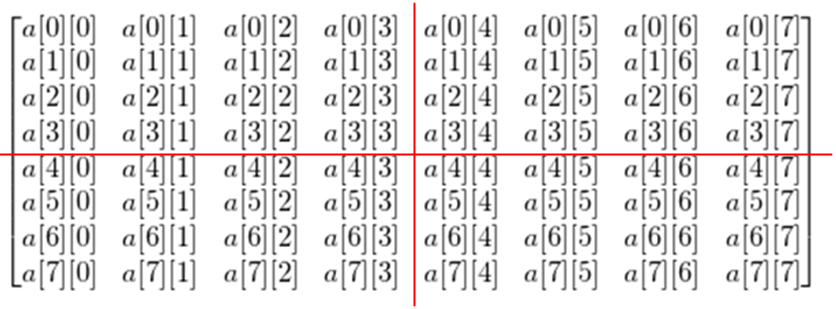
\includegraphics[scale=0.4]{Splitting.png}
\caption{An $8\times8$ matrix that is split into smaller $4\times4$ matrices}
\label{Splitting}
\end{figure}

\section{Conclusion}
\label{Conclusion}
The conclusion goes here.


\begin{thebibliography}{}

\bibitem{PThread}
Barney, B; Livermore, L; \emph{POSIX Threads Programming}; \url{https://computing.llnl.gov/tutorials/pthreads/}; Last Accessed: 01/03/2018

\bibitem{StackOverflow}
Ball, M; \emph{c - Pthreads vs. OpenMP - Stack Overflow}; \url{https://stackoverflow.com/questions/3949901/pthreads-vs-openmp}; Last Accessed: 01/03/2018

\bibitem{OpenMP}
Barney, B; Livermore, L; \emph{OpenMP}; \url{https://computing.llnl.gov/tutorials/openMP/}; Last Accessed: 01/03/2018

\bibitem{Amdahl}
Unknown; \emph{What is Amdahl's Law? - Definition from Techopedia}; \url{https://www.techopedia.com/definition/17035/amdahls-law}; Last Accessed: 02/03/2018

\end{thebibliography}




% that's all folks
\end{document}


